\chapter{Projektin lähtökohdat}
\label{ch:projektin-lähtökohdat}
Ennen tämän työn aloittamista yrityksessä oli jo kehitetty ensimmäinen versio ohjelmasta, joka kykeni tilaamaan viestejä IED-laitteelta. Prosessoimaan viestit ja tallentamaan ne relaatiotietokantaan myöhempää käyttöä varten. Tässä ohjelmistossa oli havaittuja ongelmia ja se ei myöskään tukenut kaikkia IEC 61850 -standardin viesteihin liittyviä ominaisuuksia. Tämän ohjelmiston toimintaperiaate ja siinä olleet ongelmat toimivat pohjana uuden version suunnittelulle ja toteutukselle. Tarkoituksena oli poistaa havaitut ongelmakohdat ja miettiä olisiko jokin muu arkkitehtuuri parempi kyseiseen toteutukseen. Ensimmäistä toteutusta ohjelmasta voisi nimittää ensimmäiseksi protoversioksi tai demovaiheeksi (engl. proof of consept), jonka pohjalta tultiin tekemään toimiva lopullinen versio. Tekstissä eteenpäin sanalla demoversio viitataan tähän ohjelmistoon.

Tässä osiossa pohjustetaan työn alkua lukijalle ja mistä lähdettiin liikkeelle. Mitä ongelmia demovaiheen toteutuksessa oli ja miten ne havaittiin. Demovaiheen ohjelmasta käsitellään sen arkkitehtuuria, mitkä olivat sen komponentit ja niiden toiminnallisuus. Asetettujen tutkimuskysymysten ja ongelmien kautta pyritään löytämään uudelle ohjelmiston arkkitehtuurille pohjaa ja ratkaisua siihen liittyviin päätöksiin.


\section{Demoversio ja sen toiminta}
Demoversio oli ohjelmoitu Ruby-ohjelmointikielellä. Ohjelman arkkitehtuuri oli todella yksinkertainen. Kuvassa \ref{fig:demo-architecture} on esitetty demoversion arkkitehtuuri korkealla tasolla.

\begin{figure}
	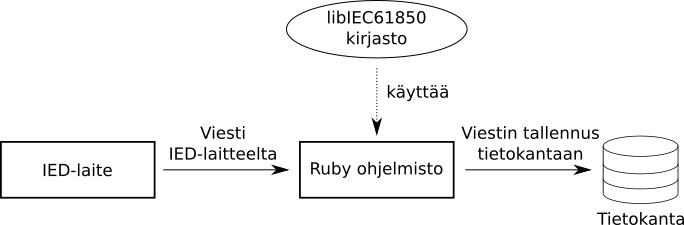
\includegraphics[width=1\textwidth]{pictures/demo-architecture.png}
	\caption{Rubylla toteutetun demoversion arkkitehtuuri ja tiedonsiirto.}
	\label{fig:demo-architecture}
\end{figure}

Yksi ajettu demoversion prosessi pystyi tilaamaan yhden IED-laitteen kaikki RCB-luokkien instanssit. Tiedon instanssien olemassaolosta ohjelma pystyi lukemaan relaatiotietokannasta. Prosessoimaan viestit ja tallentamaan ne relaatiotietokantaan myöhempää käyttöä varten. Ruby-ohjelmistossa tärkeässä osassa oli libIEC61850-kirjasto\footnote{\url{http://libiec61850.com}}. libIEC61850-kirjasto on avoimen lähdekoodin C-kielellä toteutettu kirjasto, joka abstrahoi IEC 61850 -standardin matalan tason määrittämiä palvelukutsuja ja datarakenteita helpokäyttöiseksi rajapinnaksi. Kirjasto tarjosi toiminnallisuuden IED-laitteella olevan serveriohjelmiston, sekä IED-laittetta käyttävän asiakaohjelmiston toteuttamiseen. IED-laitteen serverille kirjasto tarjosi funktioita ja rakenteita IEC 61850 määrittämien luokkien ja hierarkian rakentamiseen ja käsittelyyn. IED-laitteen asiakasohjelmalle kirjasto tarjosi funktioita ja rakenteita standardin määrittämiin palveluihin, kuten arvojen lukuun ja asettamiseen, datajoukkojen käyttöön ja viestien tilaamiseen. Tätä samaa kirjastoa käytettiin myös tämän työn toteutetussa ohjelmistossa. Koska demoversiossa ja tämän työn toteutuksessa keskitytään vain asiakasohjelmiston tekemiseen, käytetään kirjastosta vain sen asiakasohjelman toteutuksen ominaisuuksia.

Kirjasto oli rakennettu käyttämään MMS-protokollaa tiedonsiirrossa IED-laitteen ja sen asiakasohjelman välillä, kuten IEC 61850 -standardin osassa 8-1 määritetään. Kuvassa \ref{fig:libiec61850-layer-architecture} on esitetty kirjaston kerrosarkkitehtuuri asiakasohjelmalle. Kirjastoon oli toteutettu laiteabstraktiokerros (engl. hardware abstraction layer, lyhennetään HAL). HAL:in avulla kirjasto voi toimia monella eri laitealustalla, ja käyttäjä voi tarvittaessa lisätä oman HAL-implementaation. Demoversiota ajettiin Linux-käyttöjärjestelmällä, joten kirjastosta käytettiin olemassa olevaa Linux HAL toteutusta. Kuvassa \ref{fig:libiec61850-layer-architecture} on punaisella merkitty laatikot, jotka kirjaston käyttäjä voi tarjota, keltaisella kirjaston uudelleenkäytettävät MMS-protokollan osuudet ja sinisellä IEC 61850 -standardin toteuttavat osuudet. Kuvaan on merkitty vihreällä demoversioon toteutetut osuudet, eli Ruby-kielelle liitos C-kieleen ja tämän päälle Rubylla ohjelmoitu demo.

\begin{figure}
	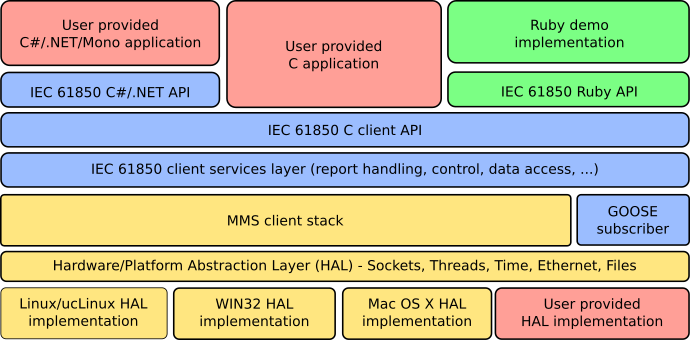
\includegraphics[width=1\textwidth]{pictures/libiec61850-layer-architecture.png}
	\caption{libIEC61850-kirjaston kerrosarkkitehruurin komponentit, vihreällä Ruby toteutukseen lisätyt osat (pohjautuu kuvaan \cite{libIEC61850-api-overview}).}
	\label{fig:libiec61850-layer-architecture}
\end{figure}

Ruby-koodista C-kielen funktioiden kutsuminen ei ole suoraan mahdollista, vaan kielten väliin täytyy toteuttaa liitos. Demoversiossa liitos oli tehty käyttäen Rubylle saatavaa ruby-ffi -kirjastoa\footnote{\url{https://github.com/ffi/ffi}} (engl. Foreign Function Interface, lyhennetään FFI). Liitoksen avulla Ruby voi kutsua C-kielen funktioita ja käyttää sen struktuureita ja muuttujia. Demossa kirjasto hoiti matalan tason IEC 61850 asiat, ja Ruby-koodi keskittyi liitoksen avulla korkean tason viestin parsintaan ja tallennukseen tietokantaan.


\section{Ongelmakohdat ja analysointi}
\begin{it}
	Kirjoita tähän osioon entisen ohjelmiston ongelmista, havannoinnista ja niiden analyysista miksi näin tapahtuu.
	Ongelmat: suorituskyky lukituksen ja GILin takia, muistivuoto railsissa, joka aiheutti muistin tasaista syömistä kokoajan, tietokannasta muiden ohjelmien pitää koko ajan lukea tietoa erikseen.

	Suorityskykyyn liittyy Rubyn GIL, libIEC61850-kirjaston semaphori lukitus. Tästä koodia teskstiin sekaan ja analyysi miksi näin tapahtuu. Voisi myös jotenkin visualisoida kuvilla. Mainintaa myös rubyn suorituksen hitaudesta tähän.
	Semaphore hal taso löytyy polusta src/hal/thread/linux/thread\_linux.c.
	Tätä käytetään IedConnection\_installReportHandler() funktiossa src/iec61850/client/ied\_connection.c:263. Ja 

	IedConnection->MmsConnection->IsoClientConnection->callback
	Säie käynnistyy kun kutsutaan IedConnection\_connect() funktiota. Säei kutsuu funktiota mmsIsoCallback(), tiedostossa src/mms/iso\_client/mms\_client\_connection.c:747.
	Säikeen funktio connectionHandlingThread() mitä ajaa on määritetty src/mms/iso\_client/iso\_client\_connection.c:120.
	Tämä funktio kutsuu mmsIsoCallback() funktiota ISO\_IND\_DATA ensimmäisenä parametrinä, mikä on ISO\_IND\_DATA ja tyyppiä IsoIndication. Tätä ei kuitenkaan nähtävästi käytetä koko funktiossa mihinkään.

	Kun RCB arvoja luetaan funktiolla getRCBValues(), niin funktio kutsuu sisäisesti sendRequestAndWaitForResponse() funktiota. Joka nukkuu ja odottaa vastausta IED-laitteelta. Jos sitä ei tule tai tulee connection timeout. Säikeen ja tämän välillä käytetään MmsConnection->lastResponseLock mutexia. Samaa funktiota kutsutaan myös sisäiseti kun RCB arvoja kirjoitetaan funktiolla IedConnection\_setRCBValues().

	Kun viestien vastaanottaja funktio asetetaan, kirjasto lukitsee mutexin IedConnection->reportHandlerMutex siksi ajaksi kunnes saa sen asetettua funktiossa IedConnection\_installReportHandler():263.

	Kun raportti saapuu IED-laitteelta, kutsutaan kirjastossa sisäisesti funktiota informationReportHandler() (src/iec61850/client/ied\_connection.c:430), mikä taas kutsuu private\_IedConnection\_handleReport() funktiota src/iec61850/client/client\_report.c:346. Tämä funktio kutsuu käyttäjän callback funktiota ja kutsun ajaksi lukitesee IedConnection->reportHandlerMutex mutexin.
	
	informationReportHandler() funktiota kutsutaan handleUnconfirmedMmsPdu(), ja tätä funktiota kutsutaan mmsIsoCallback() funktiosta, joka on ajossa erillisessä säikeessä.
\end{it}

Demoversiossa ohjelma oli toteutettu Ruby on Rails kehyksen päällä ajettavaksi. Ruby on Rails kehys on tarkoitettu web-sovellusten toteuttamiseen Ruby kielellä. Se tarjoaa Active Record nimisen ORM-kerroksen (engl. Object-relational Mapping). ORM-kerros abstrahoi relaatiotietokannan käyttämisen oliopohjaiseksi ja kyselyitä tietokantaan voi suoraan tehdä Ruby-kielellä. Demoversio käytti Railsin Active Record ORM-kerrosta tietokannan käyttämiseen. Eli ennen ohjelman ajamista ohjelmaan täytyi ladata Railsin ajoympäristö muistiin, joka aiheutti sen että yksinkertaisen ohjelman täyti varata iso määrä muistia ennen suoritusta. Linuxin htop-ohjelmalla katsottuna, prosessi varasi noin 150 Mt muistia ajoa varten.

Ohjelma luki tietokannasta IED-laitteen, sekä sen kaikki RCB-instanssien tiedot. Tietojen avulla ohjelma tiesi mikä IED-laitteen IP-osoite on ja mitkä olivat RCB-instanssien referenssit. Ohjelmaan pystyi syöttämään eri tietoja ainoastaan tietokannan kautta ennen ajoa. Tämän jälkeen ohjelman toiminta, jokaisen RCB-instanssin viestien tilaukseen ja prosessointiin on esitetty sekvenssikaaviossa kuvassa \ref{fig:sequence-diagram-report-subscription}. Kuvassa ohjelman kaksi eri silmukkaa on esitetty kahdella eri seq-laatikolla.

\begin{figure}
	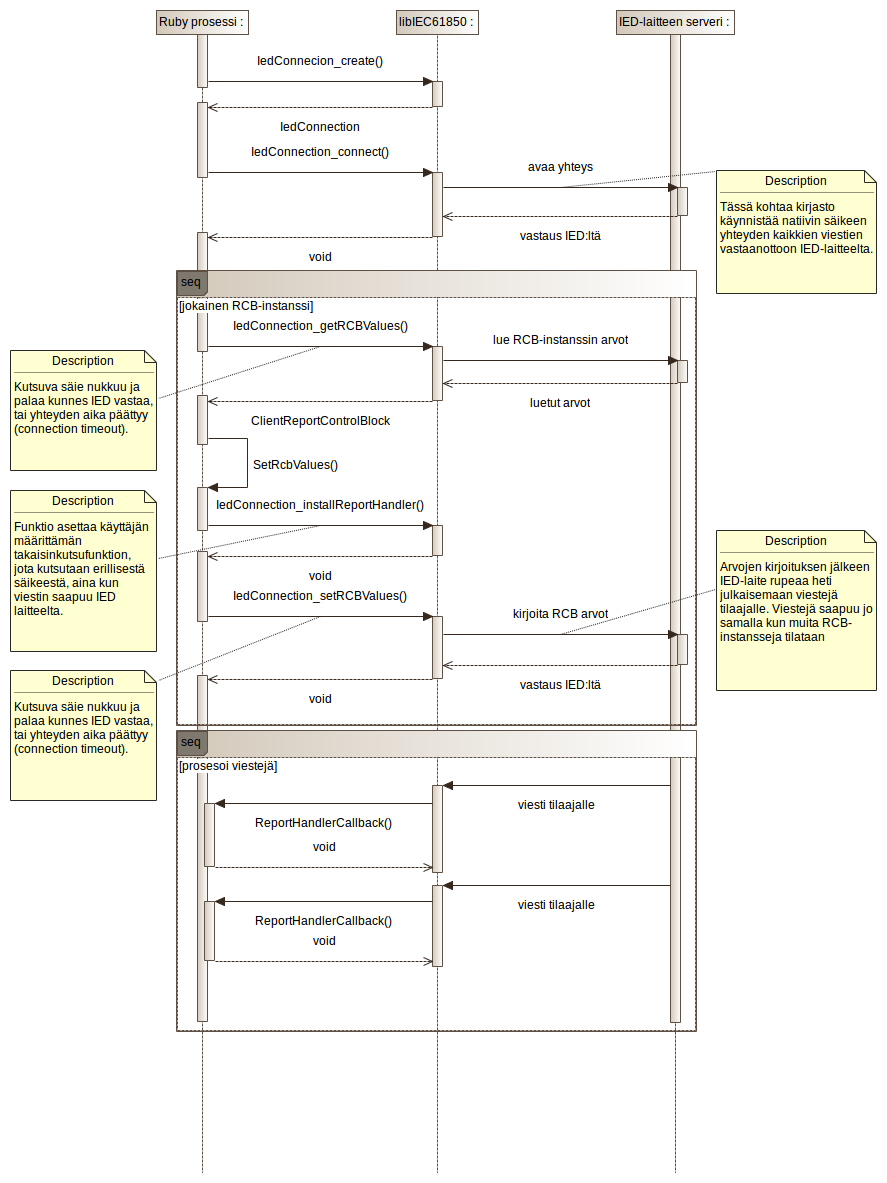
\includegraphics[width=1\textwidth]{pictures/sequence-diagram-report-subscription.png}
	\caption{Sekvenssikaavio kaikkien RCB-instanssien tilaukseen yhdeltä IED-laitteelta demo-ohjelmalla.}
	\label{fig:sequence-diagram-report-subscription}
\end{figure}

Sekvenssikaaviossa osallisena ovat Demon Ruby-prosessi, libIEC61850-kirjasto, johon liitos oli tehty ruby-ffi -kirjastolla. Ja IED-laiteen serveriohjelma, johon libIEC61850-kirjasto kommunikoi verkon yli. Sekvenssikaaviota on hieman yksinkertaistettu, esim. libIEC61850-kirjaston tekemää erillistä säiettä ei kuvata ja ruby-ffi kirjastoa ei ole merkitty lainkaan.

Tietokannasta luettujen tietojen jälkeen ohjelma muodostaa yhteyten IED-laitteelle, ensin tekemällä instanssin \texttt{IedConnection} struktuurista funktiolla \texttt{IedConnection\_create()}. Tämän jälkeen struktuuri annetaan \texttt{IedConnection\_connect()} funktiolle, joka avaa yhteyden IED-laitteelle ja palaa vasta kun vastaus saapuu. Tässä vaiheessa libIEC61850-kirjasto käynnistää erillisen natiivisäikeen yhteyden viestien vastaanottoon. Tämä tapahtuu kirjaston lähdekoodissa src/mms/iso\_client/iso\_client\_connection.c funktiossa \texttt{IsoClientConnection\_associate()} riveillä 429--434. Tätä säiettä kirjasto käyttää tulevien viestien vastaanottoon ja lähettämiseen. Yhteyden avauksen jälkeen jokainen RCB-instanssi tilataan lukemalla ensin sen arvot IED-laitteelta funktiolla \texttt{IedConnection\_getRCBValues()}. Funktiokutsu nukkuu ja palaa vasta kunnes erillinen säie ilmoittaa että vastaus on saapunut, tai yhteyden aika ylittyy. Kirjaston funktio, joka tämän hoitaa on \texttt{sendRequestAndWaitForResponse()} ja on määritetty src/mms/iso\_mms/client/mms\_client\_connection.c riveillä 345--418. RCB-arvot luettuaan, kirjasto palauttaa struktuurin \texttt{ClientReportControlBlock}, joka sisältää luetut tiedot RCB-instanssista. Samaa struktuuria käytetään arvojen muuttamiseen ja niiden takaisin kirjoittamiseen IED-laitteelle. Ennen muunneltujen RCB-arvojen takaisin kirjoittamista ja viestien tilaamista, täytyy kirjastolle asentaa takaisinkutsufunktio, jota kirjastoo kutsuu aina kun tilattu viesti saapuu IED-laitteelta. Takaisinkutsufunktio asetetaan \texttt{IedConnection\_installReportHandler()}, joka ottaa parametrikseen funktiopointterin ja vaihtoehtoisen parametripointterin. Heti arvojen kirjoitusten jälkeen IED aloittaa lähettämään viestejä. TODO: finish up


\section{Puuttuvat ominaisuudet}
\begin{it}
	Kirjoita tähän mitä puuttuvia ominaisuuksia demoversiossa oli ja mitä vaatimuksia uuteen toteutukseen pitäisi olla. listaa niistä olisi hyvä ja miten demoversio ei niitä täytä.
	
\end{it}
Ohjelmisto pystyi tilaamaan ja vastaanottamaan raportteja yhdeltä IED:ltä ja siinä monelta määritellyltä RCB:ltä. Ohjelmisto prosessoi ja tallensi raportteja tietokantaan muuta käyttöä varten. Tilanteessa, jossa raportteja tilaavassa järjestelmässä on monta osaa, jotka kaikki tarvitsevat raporttien tietoja reaaliajassa. Joutuvat eri osat tässä tilanteessa kyselemään tietoja tietokannasta, ilman erillistä tietoa niiden saapumisesta. Tämä aiheuttaa turhaa kuormaa tietokannalle ja tietojen saaminen reaaliajassa ei ole mahdollista. Myöskin jos komponentti tarvitsee tietyn tyypin raportteja, ei kaikkea tietoa, ongelma on sama.

Ohjelmiston suorituskyky paikoin raporttien määrän ollessa suuri aiheutti ongelmia. Syynä Rubyn toteutuksessa oli oletustulkissa (\emph{CRuby}) oleva globaali lukitus (engl. \emph{Global Interpreter Lock}, \textbf{GIL}). Vaikka Rubyn säie on oma käyttöjärjestelmän tarjoama säie, GIL estää säikeiden yhtäaikaisen suorituksen ja vain yksi säie on suorituksessa kerrallaan \mbox{\cite[s.~131--133]{Odaira2014}}. Linux-pohjaisella käyttöjärjestelmällä libIEC61850-kirjaston laitteistoabstraktiokerros (engl. \emph{Hardware Abstraction Layer}, \textbf{HAL}) käyttää POSIX-säikeitä \cite{libIEC61850-repo}. Linux-käyttöjärjestelmän säikeet ovat suorituksessa yhtä aikaa ja moniytimisellä prosessoreilla asioita tapahtuu samalla ajan hetkellä. Nyt raportin saapuessa, C-prosessin säikeen suoritus kutsuu takaisinkutsuntaan asetettua funktiota, joka on implementoitu Rubyn puolella. On funktion suoritus GILin alaista suoritusta. Ruby-prosessin myös suorittaessa muuta toimintaa takaisinkutsujen välissä, on Rubyn suorituskyky ohjelmiston pullonkaulana raporttien määrän ollessa tiheää.

\begin{it}
	Kirjoita tähän vielä ongelmasta kun tilataan monta RCB:tä. Raporttien tullessa Rubyn puolelle, ei Rubyn muu koodi saa tilattua loppuja RCB:tä kirjaston lukitusten takia. Ja yhteys aikakatkeaa tämän takia. Selitä lukituksista tarkemmin ja myös liitä pätkiä libIEC61850-kirjaston koodista. Syyn selityksen voi siirtää muualle. Kirjoittaa vain että on ongelma, ja selvitys miksi, muualla.
\end{it}